\section{Methods}
\label{sec:methods}
To test our hypothesis, we constructed a simple, two-layer recurrent neural network (based on Aungiers, 20184). For data, we used publically available pricing data from the AWS spot market. Effectiveness was measured by how well our network could predict the next spot price. 
We developed two workflows, one as a baseline and one as a test case (illustrated to the right). The RNN was constructed using Keras with a Tensorflow back-end and the workflows were completed using this implementation within a Python notebook. Each workflow was run 10 times in order to ensure accuracy and reproducibility.
The baseline workflow simply trains our neural network from N different initialization and then choses the trained model with the lowest loss after K epochs. This is effectively the same as retraining a number of times to find a trained model with the best parametrization.
Our experimental workflow begins in the same manner as the baseline workflow. However, during the training (for example, after K/2 epochs), optimization is halted and only the top T networks are selected. We then merge the weights of the two networks using some predefined function, an illustration of which is pictured to the right. We then re-spawn N networks with slight random mutations between them and continue training until we have reached K epochs.

\begin{figure}[h!]
\begin{subfigure}[h]{0.49\linewidth}
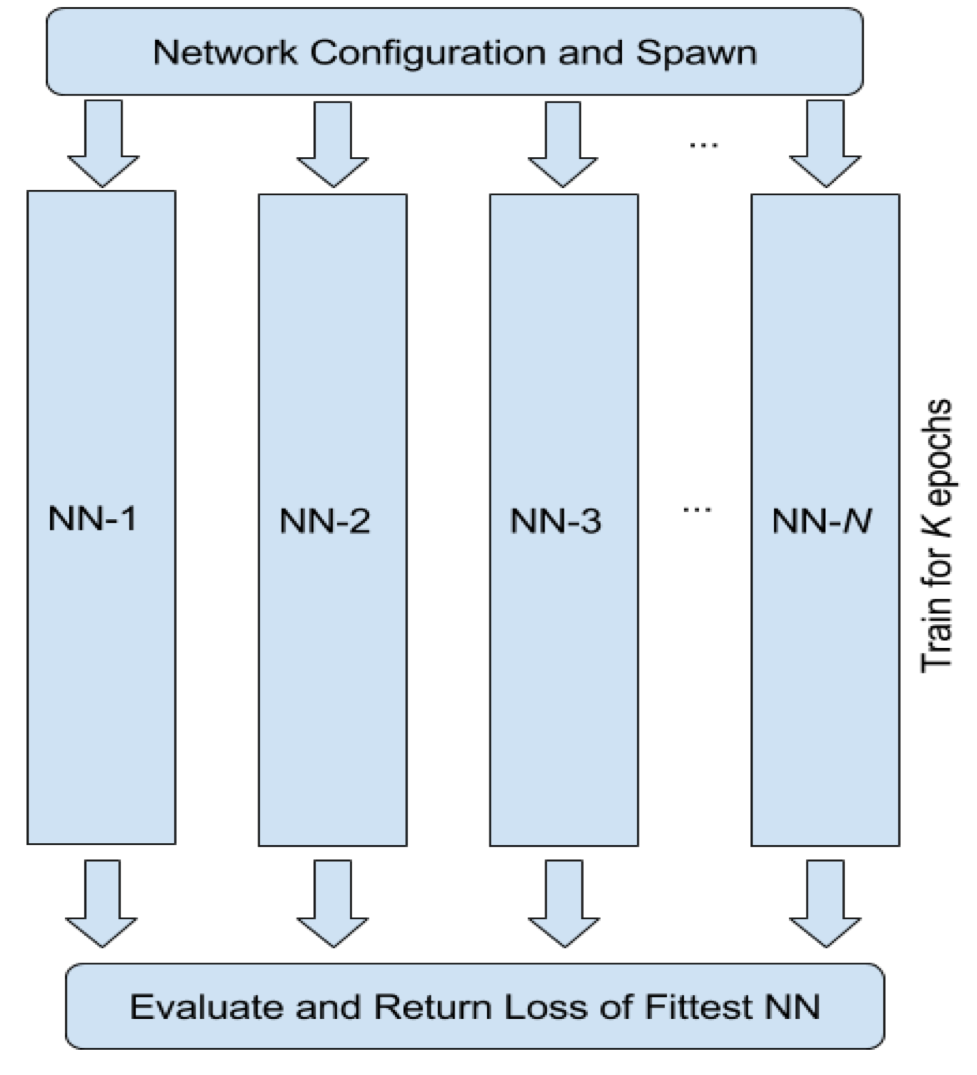
\includegraphics[width=\linewidth]{figures/simple.png}
\caption{Control, no cross-over.}
\end{subfigure}
\hfill
\begin{subfigure}[h]{0.49\linewidth}
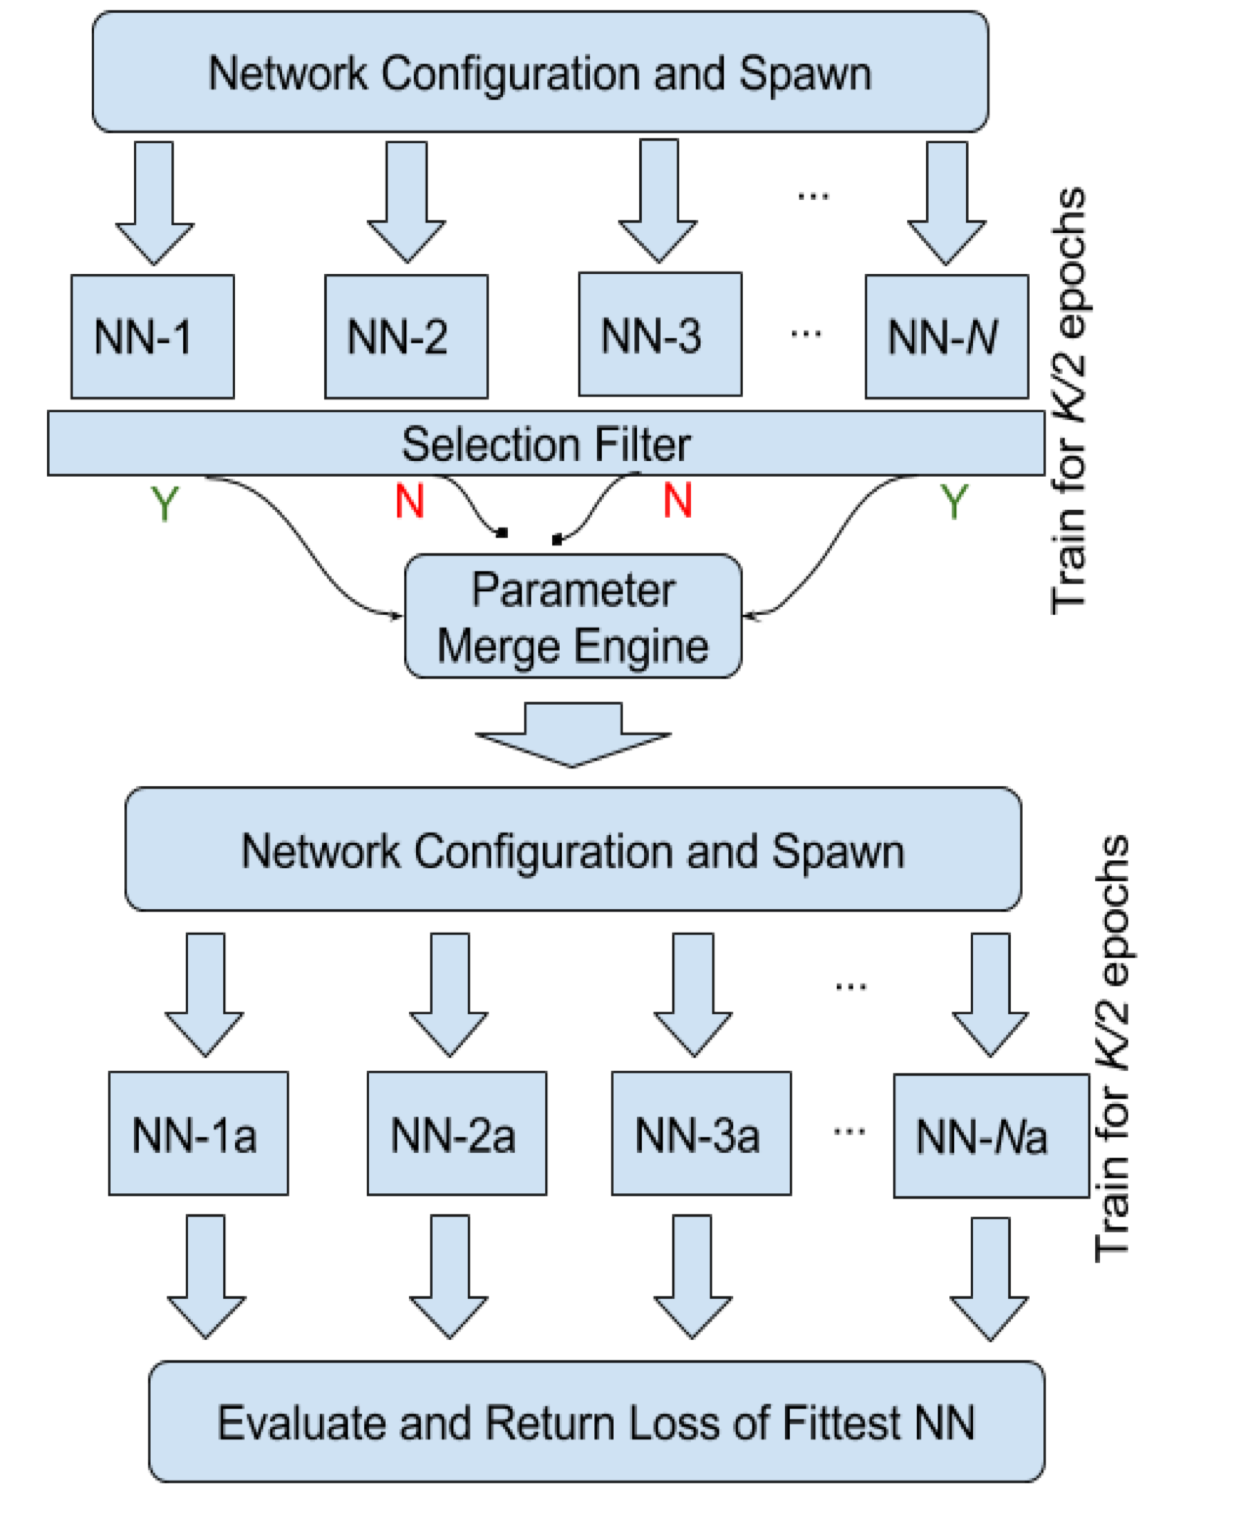
\includegraphics[width=\linewidth]{figures/workflow.png}
\caption{Test, with cross-over.}
\end{subfigure}%
\caption{Generalized control and test workflows used to evaluate parameter merging.}
\end{figure}

\begin{figure}[h!]
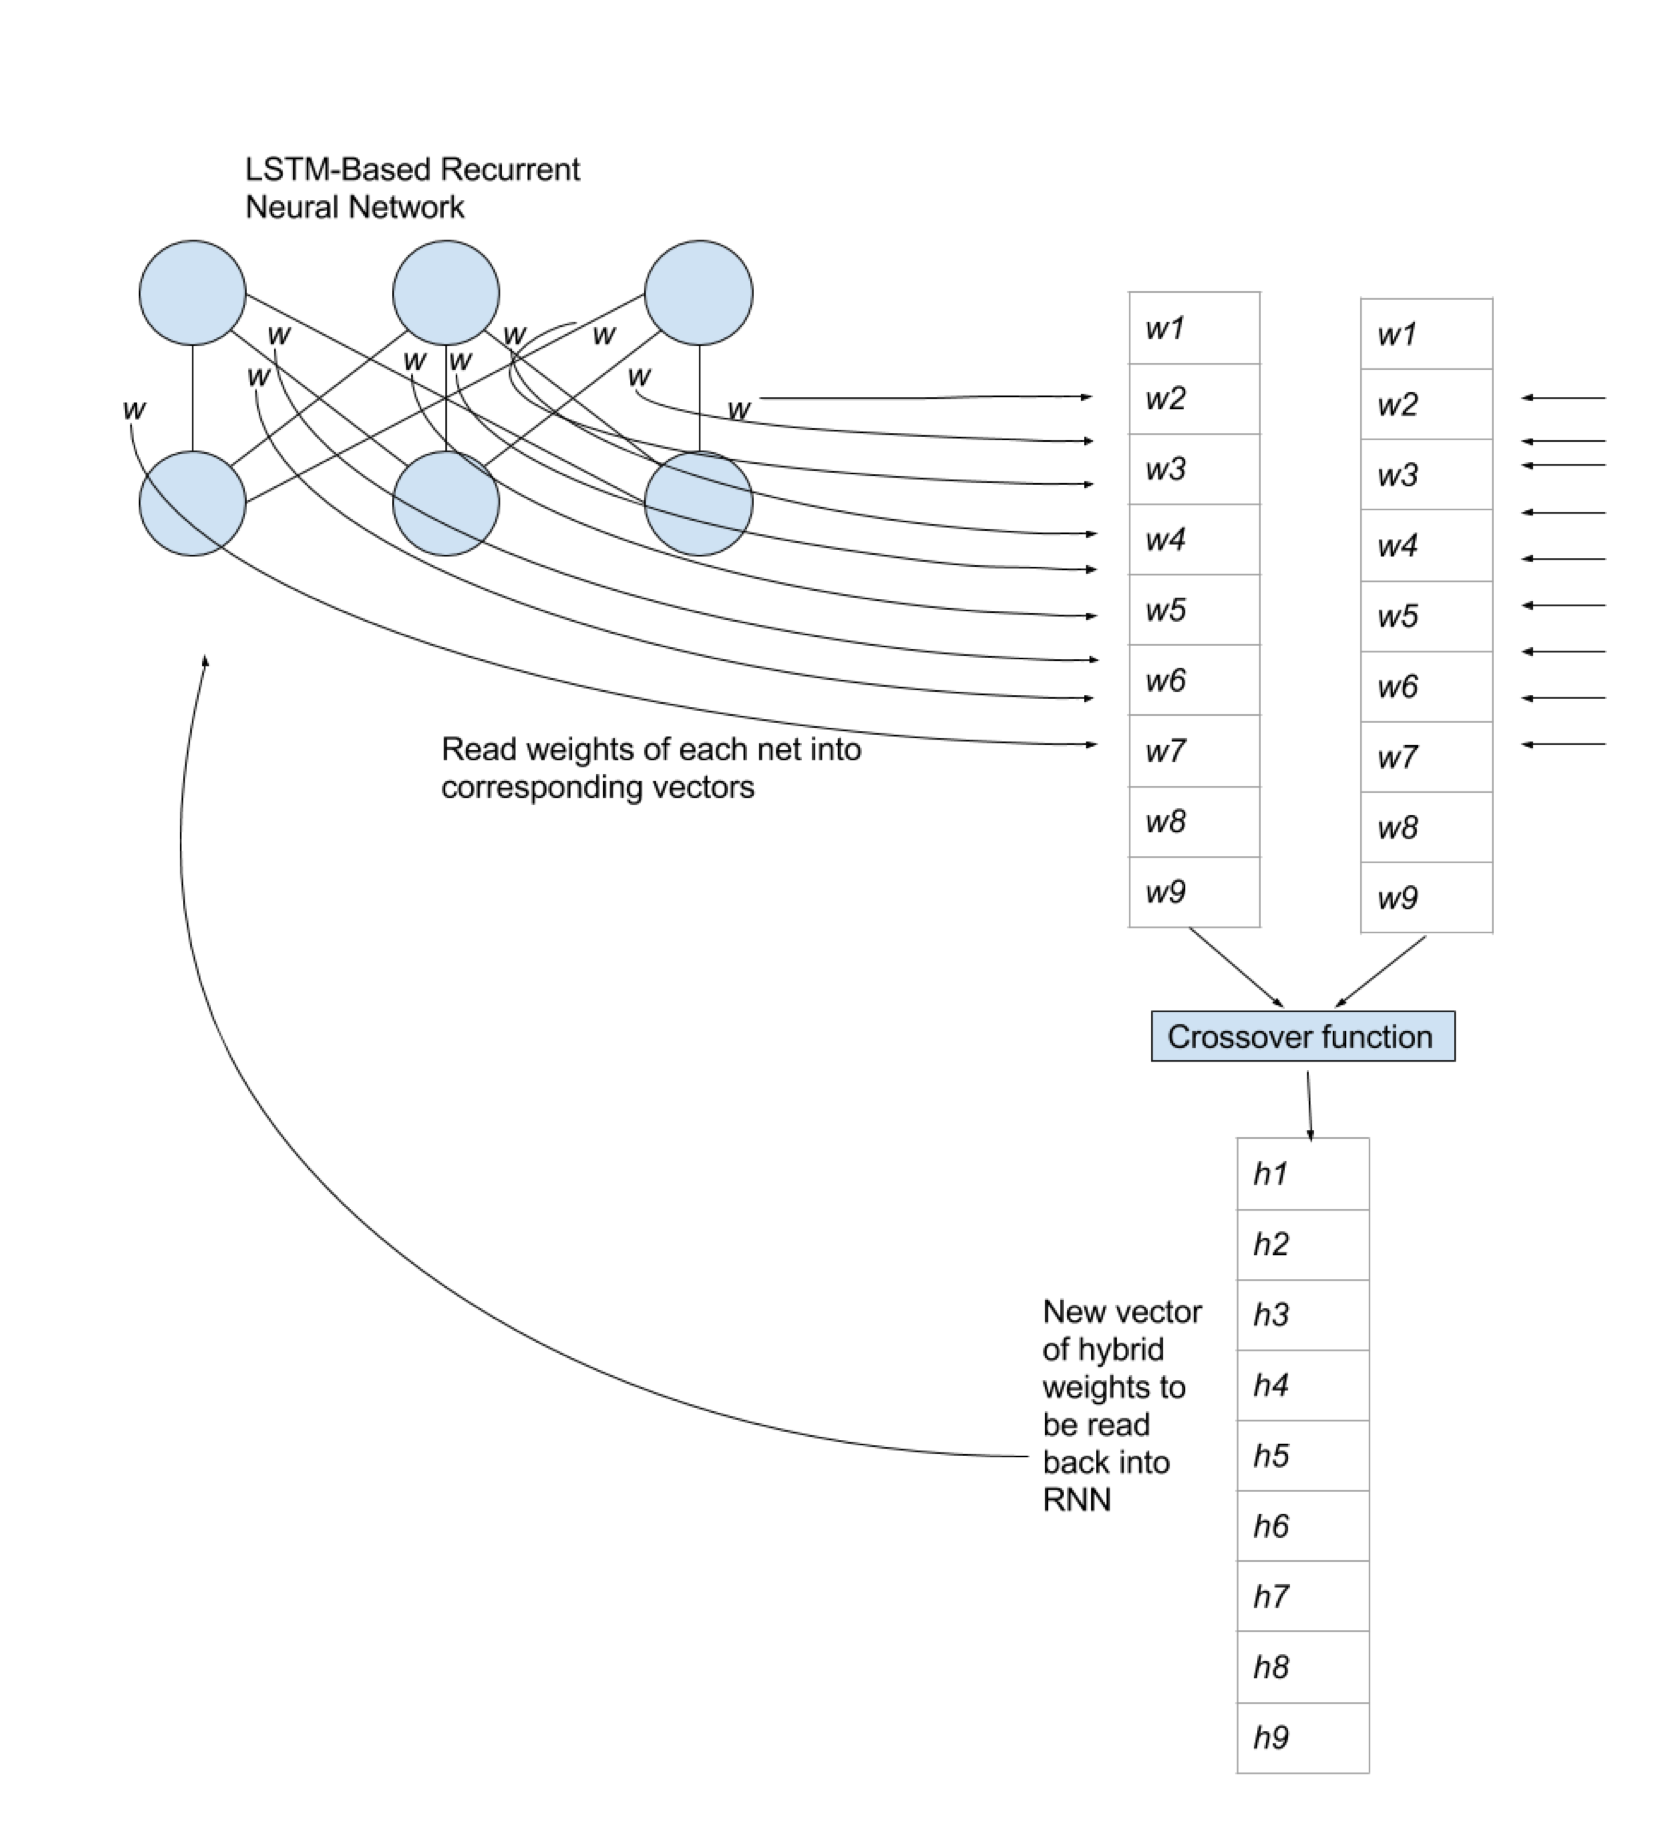
\includegraphics[width=\linewidth]{figures/merge.png}
\caption{Illustration of merging network weights}
\end{figure}